\documentclass[a4paper,12pt]{article}
\usepackage{enumitem}
\usepackage{graphicx}
\usepackage{placeins}

\renewcommand{\thesubsection}{\thesection\alph{subsection}}


\begin{document}

\title{Intro to AI Project 1}
\author{Tim Raymaker and Mike Rizzo}
\date{\today}

\maketitle

\section{Part 1: Understanding the Methods}

\subsection{}
The agent will move toward the cell with the lowest $f$-value. The $f$-value is determined from the sum of the cost from the start, or $g$-value,  and the heuristic value to the goal, or $h$-value. For the first move, each possible direction is one tile away from the start, meaning that the $g$-value for each move will be the same, and differences in the $h$-value will be the deciding factor on where to move. Since the agent does not know that cells D3 and E4 are blocked, it will move to the east, the direction that leads to the cell with the lowest $h$-value and therefore the lowest $f$-value. 

\subsection{}
The answer has been divided into four cases:
\begin{enumerate}
	\item Case 1: The agent can find the target and the target is reachable.
		\newline The agent will go about expanding nodes that lead it closer and closer to the target until eventually it will encounter the target and stop. 
		
	\item Case 2: The agent can tell there is no solution when the target in unreachable.
		\newline
		
	\item Case 3: The agent makes upper-bounded number of moves when the target is reachable.
		\newline
		
	\item Case 4: The agent makes an upper-bounded number of moves when the target is unreachable.
		\newline
		
\end{enumerate}

\section{Part 2: The Effects of Ties}
We observed for that favoring a high or low $g$ in the case of a tie value had little to no effect on the performance of the Repeated Forward A* search. On average, the runtime for favoring low $g$ was ~5.84 seconds. Favoring high $g$ was nearly identical, being slower on average only by a hundredth of a second at ~5.86 seconds. Investigating further, we see the median Though our runtimes were nearly identical, using g to tiebreak would likely be useful for performance on an empty map as it would help limit expansions. In the maps provided, the amount of obstacles in the way means that there is relatively little gain with manipulating $g$.
 	
\section{Part 3: Forward vs. Backward}
The Repeated Forward A* search and Repeated Backward A* search were both able to find possible solutions, where solutions existed, but their exact paths differed in most cases. The difference comes from the difference in path planning and replanning. Because backward plans from the goal, different blocked and unblocked cells are found at each iteration. Neither method’s path was consistently superior to that of the other. 

\section{Part 4: Heuristics in the Adaptive A* (i)}
The "Manhattan Distance" can be described as the number of moves required to reach a goal given no obstacles. Therefore, it makes sense that said distance will be consistent. If an h-value in adaptive A* becomes inconsistent, it is because something is in the way. In this case, the heuristic will be updated and will become consistent again. \newline
Given a node s and neighbor m: \newline
%INCOMPLETE: PROOF OF ADAPTIVE H-VALUE

\section{Part 5:  Heuristics in the Adaptive A* (iI)}

\section{Part 6: Memory Issues}

\subsection{Improvements to Our Implementation}
We currently use Python's tuples to record $(x , y)$ coordinate information. According to Python's "sizeof" function, for one, 2-integer tuple, the memory consumption is 40 bytes. We could reduce this by storing the coordinates in the minimum number of bits it takes to store two $0 \rightarrow 100$ values. We could then also keep the tree pointers on two bits with the binary values 

\subsection{Calculations}
(1,001 x 1,001) = 1002001 cells \newline
At 2 bits per cell: \newline
2 * 1002001  = 2,004,002 bits ~ 250 kB \newline \newline

4MB = 32000000 bits \newline
At 2 bits per cell: \newline
	16000000 cells possible \newline 
	grid size = sqrt(16000000) = 4000 x 4000 grid

\section{Data, Methods, and Observations}

Data was collected for Repeat Forward A* with Tie-breaking in favor of Low $g$-values, Repeat Forward A* with Tie-breaking in favor of High $g$-values,  Repeat Backward A* with Tie-breaking in favor of Low $g$-values, Repeat Backward A* with Tie-breaking in favor of High $g$-values, Adaptive A* with Tie-breaking in favor of High $g$-values algorithms. The searches were each performed on the 50 maps generated in Part 0. The start and end goal were standardized to $(0,0)$ and $(100,100)$. Of the 50, 26 had solutions. The 24 without solutions are marked in red and their runtimes are not included in the data because animation conflicted with reporting significant and comparable runtimes. For each of the 5 algorithms, we have calculated and provided a median and mean runtime. These values are recorded in the Figure 1:

\begin{figure}[!htbp]
	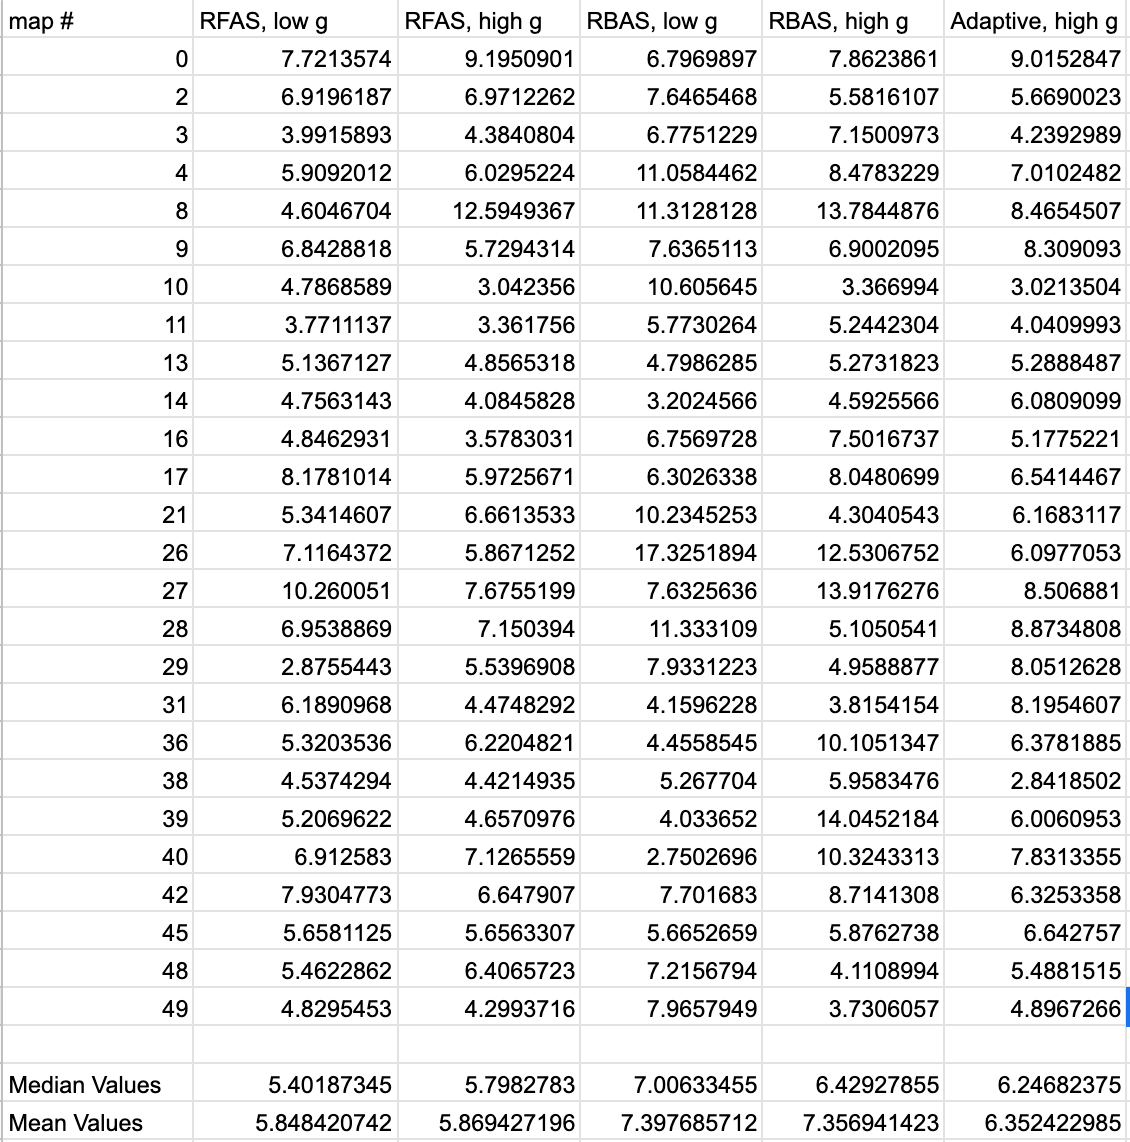
\includegraphics[angle=0, origin=c, width =  0.68\textwidth]{data1.jpg}
	\caption{Our Data}
\end{figure}
\FloatBarrier

Sources of error can be attributed to small sample size and random choices in cases of $g$-values also tying. If there were more time, we would have like to address the small sample size by generating more graphs that tested specific edge cases as well as graphs at varying amounts of blockages. As well, the randomization in the implementation can lead to variance in the paths taken and nodes expanded even by the same search on the same map. Finally, optimization differences between different hardware and software may also have played a role in the uniformity of our data. We acknowledge these issues and have answered the as best as possible. 

\end{document}

======
\section{Part 2}
Tie-breaking was important in the planning phase of the A* search. Tie-breaking in favor of low $g$-values meant prioritizing tied neighbors that were closer to the start in the heap. Tie-breaking in favor of high $g$-values meant the opposite. From our data, Tie-breaking in favor of low $g$-values was able to find very slightly shorter paths in slightly shorter times than high-g was. This seems counterintuitive, given that in the example problem a high-g search will drastically outperform low-g by cutting straight to the goal where low-g explores other nodes, but it is worth considering that high-g's worst case was often worse than low-g's. High-g searches favored diving toward the goal, which for an uncluttered map is optimal, but our map had enough obstacles that every search was significantly hampered. High-g, in its attempt to 'greedily' find a solution as fast as possible, sometimes ended up trapped in dead end areas with no way forward, being forced to backtrack significantly. Low-g, on the other hand, performed a slower but safer search. In this example low-g is more akin to BFS while high-g played a similar role to DFS. Of course, the average and best case scenarios of high-g are much better than those of low-g. With more maps and more data, perhaps a higher density of average cases would have shown high-g to perform better overall. \newline
To see average runtimes as well as average solution length, see end of report.
\section{Part 3}
The Repeated Forward A* search and Repeated Backward A* search were both able to find possible solutions where solutions existed, but their exact paths differed in some cases. This is likely because that although they solved the same maze, each one had different information available to them as they could only see cells near them. As such, their differing starting locations led them down different paths. Neither method’s path was consistently superior to that of the other, but the backwards paths tended to have worse runtimes, perhaps due to the fact that we only animated the projected paths of A* in the first quadrant. Although the forward searches would have longer projected paths, the amount of replans for the backward searches was likely higher in the first quadrant as the searches neared their goal and the amount of available moves became more limited.


\section{Part 5}
Our adaptive A* method was able to find shorter paths than forward A* on average, but it also took a longer time. This is likely due to it attempting to avoid previous projected paths and move in new directions. Our A* recalculated the heuristic value of every tile that was expanded by the previous A* search upon replanning, increasing their cost by using g(sgoal)-g(s) and incentivising the algorithm to explore alternatives.  By doing so it was sometimes able to find a better path at the cost of runtime. Ties were broken randomly and each search weighed in favor of larger g values.
\section{Part 6}
Our tree pointers pointed to a tuple coordinate, but changing them to point in a specific direction would decrease memory costs. Changing the method of visualizing the path of the agent would also likely yield a reduction in memory consumption. In order to illustrate the projected paths of the algorithm, we repeatedly filled in lines of boxes using pygame. Eliminating unecessary animation would streamline the program. The binary heap and use of tuples and Python dictionaries was fairly cost effective. Improving upon the A* algorithm outlined in the project description could also reduce runtime and memory usage. Plotting the entire path of the agent with each replan is inefficient when the agent is usually stopped after only a few moves. Planning a shorter path and replanning if necessary might be helpful. \newline
